% Chapter 4
\chapter{Optical Character Recognition} % Main chapter title

\label{Chapter4} % Fr referencing the chapter elsewhere, use \ref{Chapter1} 

\lhead{Chapter 4. \emph{Optical Character Recognition}} % This is for the header on each page - perhaps a shortened title

%----------------------------------------------------------------------------------------
\section*{Overview}
Tucked with mathematical preliminary necessary for understanding the intuition behind manifold learning, we discussed the representative manifold learning algorithms in detail. In this chapter, we now move on to some real application called optical character recognition. We motivate the importance of manifold learning algorithms discussed in chapter \ref{Chapter5} through  dimensionality reduction, clustering and classification of digits from the MNIST database of handwritten digits. %----------------------------------------------------------------------------------------

\section{Introduction}
\label{C4:Intro}

The problem of classification of the digits is perhaps one of the most widely studied among machine learning communities. Among the classification task, optical character recognition have found applications in bank check processing, assistive technology for visually impaired users, automatic number plate recognition and many more. The initial excitement over deep learning methods was triggered by their success on the MNIST handwritten digit recognition problem \citep{LeCun1998}, which was for several years the standard benchmark problem for hard, large dataset machine learning. A basic requirement for credibility of classification algorithms  requires a high accuracy on MNIST datasets.

In this chapter \ref{Chapter4}, we intend to apply various manifold learning algorithms to the MNIST data set of handwritten digit images. The global plan is to evaluate manifold learning algorithms to better understand how the classification algorithms perform under the lens of curse of dimensionality. Our goal is to automatically determine what a handwritten digit image ranging from 0 to 9. The earlier experimental results doing comparison between different manifold learning algorithms shows that these methods can work pretty well at least in our toy examples. We show this results using readily available code from Matab and Python in Appendix \ref{AppendixA}.

\section{Data}
\label{C4:data}

The standardised MNIST database has a training set of 60,000 examples, and a test set of 10,000 examples. The images contain grey levels as a result of the anti-aliasing technique used by the normalization algorithm. Then after, the images were centered in a $28\times28$ image by computing the center of mass of the pixels, and translating the image so as to position this point at the center of the $28\times28$ field. As a result, each example is of size $28\times28$, a total of 784 greyscale pixels. If we take training set, we  60,000 rows (images) and 785 (784 pixels and a one label) columns. Each row component contains a value between one and zero and this describes the intensity of each pixel. On the another hand, the test set is identical to the training set except that it is unlabeled, and so only contains 784 columns instead of 785.  The data is quite popular amongst machine learning communities because it requires minimal efforts on preprocessing and formatting. It is the de facto 'hello world' dataset of image processing and computer vision. 

\section{Prepossessing}
\label{C4:prepos}
The first step in any data science project is data visualization. First 50 training examples can be observed in figure \ref{4_1} after dropping labels.

\begin{figure}[h!]
\begin{center}
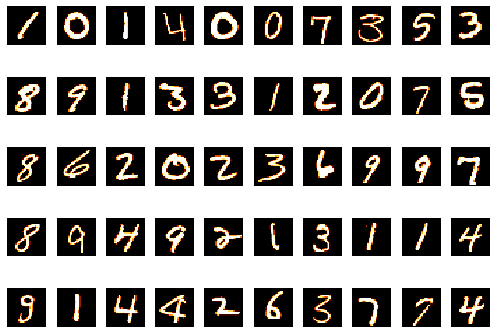
\includegraphics[width=\textwidth]{./Figures/4_1.png}
\caption {First look at MNIST data}
\label{4_1} 
\end{center}
\end{figure}

Figure \ref{4_1} revels some interesting facts about the data. Very close but important observation shows that there is a lot of the bordering pixels having black color. We also see that a few of the depicted digits are skewed. Although, MNIST datasets are already preprocessed, but there is always scope for massaging the data better. The obvious choice to vertically align the skewed digit is Hough transform \citep{Lean2008}. The purpose of the Hough transform is to find imperfect instances of objects within a certain class of shapes by a voting procedure. This voting procedure is carried out in a parameter space, from which object candidates are obtained as local maxima in a so-called accumulator space that is explicitly constructed by the algorithm for computing the Hough transform. We apply Hough transform to training data yielding vertically aligned digits except some, which were not aligned. Figure \ref{4_2} illustrates the former discussion. We are not sure that Hough transform will increase our efficiency, but we just wanted to try considering it might have some positive effect on classification accuracy.

\begin{figure}[h!]
\begin{center}
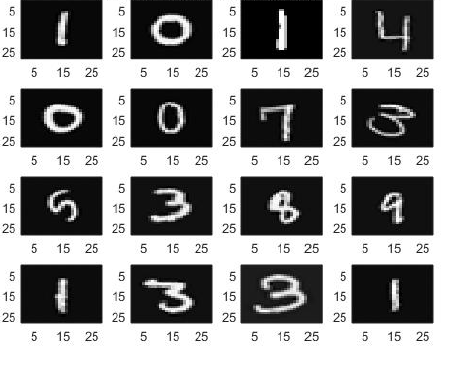
\includegraphics[width=\textwidth]{./Figures/4_2.png}
\caption {Hough transform}
\label{4_2} 
\end{center}
\end{figure}

\section{Experiments and Results}
\label{C4:ER}

With prepossessed data in our hand, we go for traditional Pearson Correlation plot in-search of meaningful insight through figure \ref{4_3}.

\begin{figure}[h!]
\begin{center}
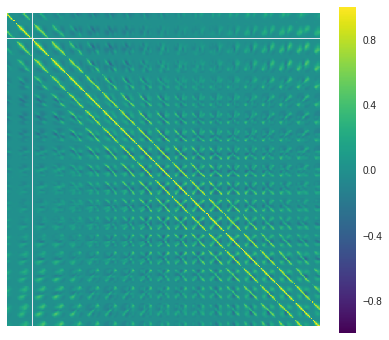
\includegraphics[width=\textwidth]{./Figures/4_3.png}
\caption {Pearson Correlation plot 500 observations}
\label{4_3} 
\end{center}
\end{figure}

The Pearson Correlation plot didn't give information due to shear size of the data. As the data is still large, we apply dimension reduction.

\subsection{Principal Component Analysis (PCA)}
PCA is a widely used linear technique in image processing. It is used for simplifying a multidimensional dataset to lower dimensions for analysis, which is essential for visualization and image processing. The data is represented in a new coordinate system using PCA, in which basis vectors
follow modes of greatest variance in the data. The mathematical details of the same is discussed in \ref{s:pca}. The graphical illustration is provided in the figure \ref{s:4_pca}.

\begin{figure}[h!]
\begin{center}
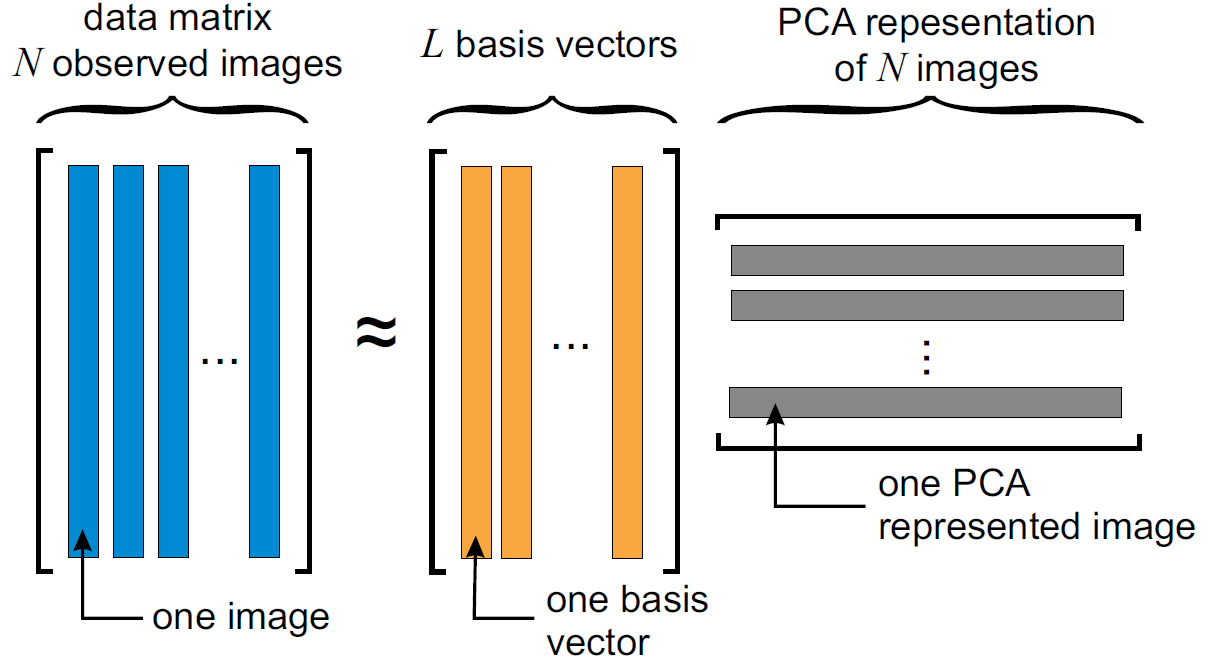
\includegraphics[width=\textwidth]{./Figures/4_pca.png}
\caption {PCA graphical illustration}
\label{s:4_pca} 
\end{center}
\end{figure}

After prepossessing of the data, the important information is to observe how the variances look like for the digits in the MNIST dataset. We take the hep of PCA to calculate the eigenvectors and eigenvalues of the covarience matrix. Working with python allows us to use standard library  to ease our work. We first standardize the data, then calculate the eigenvectors and eigenvalues of the covarience matrix. After shorting it, we calculate  explained Variance from the eigenvalues depicted in the figure \ref{pca_var}.

\begin{figure}[h!]
\begin{center}
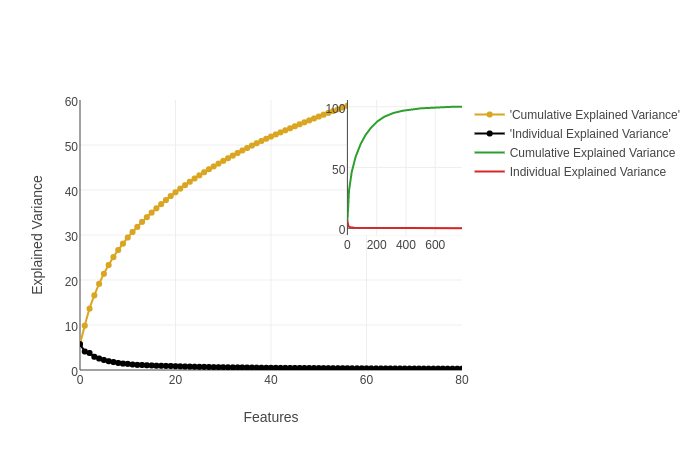
\includegraphics[width=\textwidth]{./Figures/pca_var.png}
\caption {Explained Variance}
\label{pca_var} 
\end{center}
\end{figure}

The distribution of the Individual and Explained variances across all features  is shown in smaller picture embedded. The larger plot represents the explained variances only. It is evident from the figure \ref{pca_var} that out of our 784 features, only 200 approximately describes 90\% of the explained variance. Now fitting data in PCA with 200 eigenvalues, we try to obtain the optimal eigenvectors/direction that captures the most variance. We do visual comparison of the top 5 eigenvalues to some of the other smaller ones using the figure \ref{pca_vis}. It is evident from the figure \ref{pca_vis} that more complicated directions are being generated in the search to maximise variance in the new feature subspace.

\begin{figure}[h!]
\begin{center}
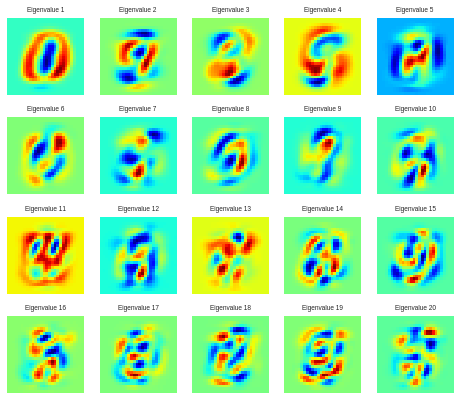
\includegraphics[width=\textwidth]{./Figures/pca_vis.png}
\caption {Top 200 eigenvalues}
\label{pca_vis} 
\end{center}
\end{figure}

We finally use dimension reduction using PCA in search of existing clusters if there is any. If seek the help from scatter plots to see the embedding using two components. The output is depicted in figure \ref{pca_dr}. As observed from the scatter plot, we don't see any clusters. This means that, for our data, the linear method, PCA is not best fit.
\begin{figure}[h!]
\begin{center}
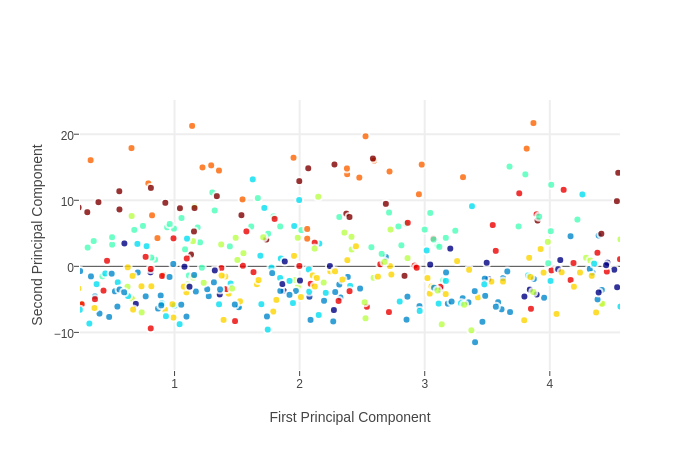
\includegraphics[width=\textwidth]{./Figures/pca_dr.png}
\caption {PCA}
\label{pca_dr} 
\end{center}
\end{figure}

\subsection{Manifold Learning}
Manifold learning is widely used in visualization, classification, and information processing of the data embedding in lower dimension.  Among all, data visualization is one of the most important method which uses 2D or 3D representation to give further insight into the data structure. This in turn can be used for either interpretation, data reduction and data model selection for extracting meaningful features from cumbersome representations. 

For our MNIST dataset, we witnessed that linear method like PCA is not good choice. Manifold learning algorithms as discussed in chapter \ref{Chapter3} provides means of data reduction by low dimensional manifold embedded in a high dimensional space. We use  t-Distributed Stochastic Neighbour Embedding (TSNE), a manifold learning algorithm introduced by van der Maaten and Hinton 
\citep{Van2008}. TSNE aims to convert the Euclidean distances between points into conditional probabilities, where student-t distribution is then applied. This serves as metrics to calculate the similarity between one datapoint to another. The scattered plot of the first two components in new feature space is illustrated in figure \ref{tsne}. It clearly identifies clusters in well defined and segregated manner. A  good cluster visualisations is prossible because of the topology-preserving attributes of the algorithm.

\begin{figure}[h!]
\begin{center}
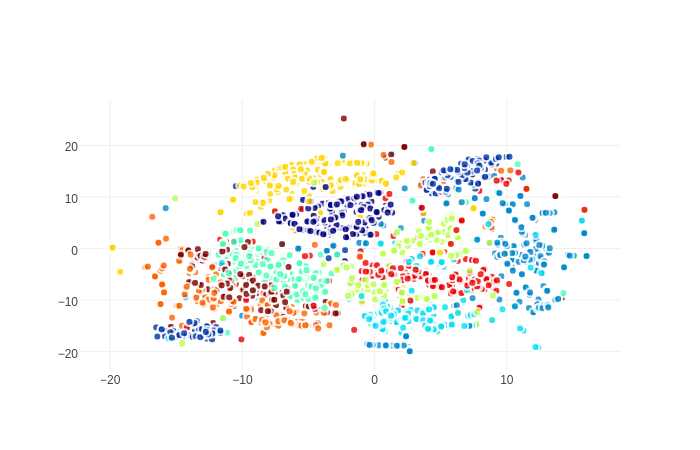
\includegraphics[width=\textwidth]{./Figures/tsne.png}
\caption {TSNE ( t-Distributed Stochastic Neighbour Embedding )}
\label{tsne} 
\end{center}
\end{figure}

We now automate the whole process and apply Isomap, Locally Linear Embedding, Spectral Embedding, Local Tangent Space Alignment, Multi-dimensional Scaling, t-distributed Stochastic Neighbor Embedding on the data to see geometric structure embedded in two dimension, represented through figure \ref{AML}. There is problem with the data or data samples we are using, as some methods fails (Local tangent space alignment). Adding to the same, the embedding of the data in lower dimension didn't give much information too.

\begin{figure}[h!]
\begin{center}
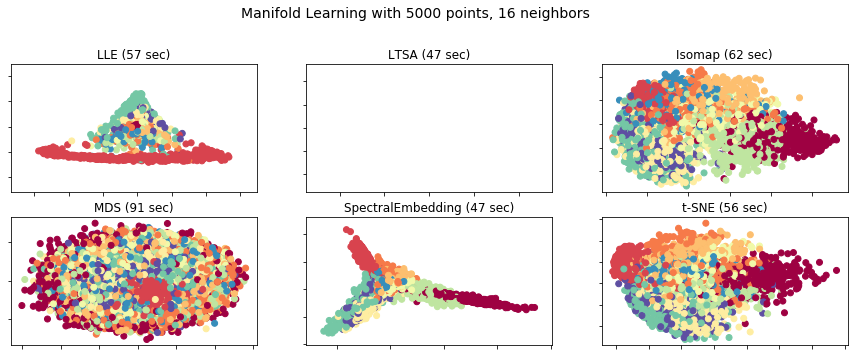
\includegraphics[width=\textwidth]{./Figures/AML.png}
\caption {Manifold Learning Algorithms Output}
\label{AML} 
\end{center}
\end{figure}

To see how manifold learning algorithms have performed, we apply out of sample for manifold learning algorithms for arbitrary point, which gives us clear pictures about clusters in the low dimensions. The figure \ref{OSML} clearly indicates that test points represented by colored dots, cross and star are projected on the area concentrated to train points. But the projection of the test points is not so clear. Separation of some numbers are blurred and not separated accurately on the manifold.

\begin{figure}[t!] % "[t!]" placement specifier just for this example 
\begin{subfigure}{0.32\textwidth}
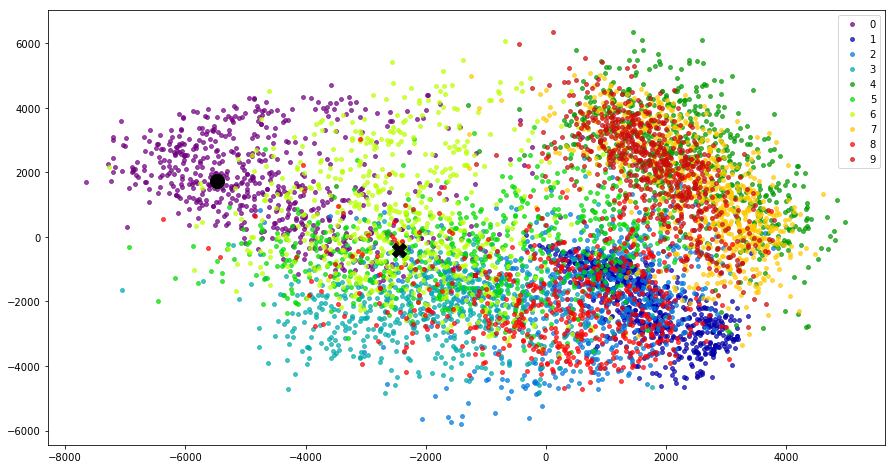
\includegraphics[height=5cm,width=5cm]{./Figures/LLE_OS.png}
\caption{LLE} 
\end{subfigure}\hspace*{\fill}
\begin{subfigure}{0.32\textwidth}
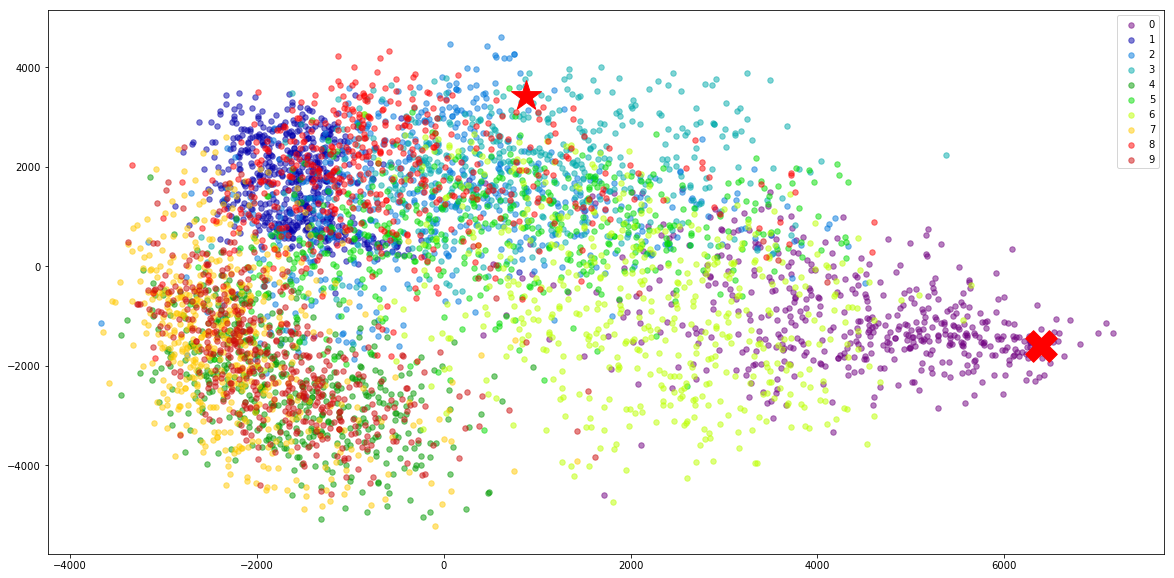
\includegraphics[height=5cm,width=5cm]{./Figures/ISO_OS.png}
\caption{ISOMAP} 
\end{subfigure}

\medskip
\begin{subfigure}{0.32\textwidth}
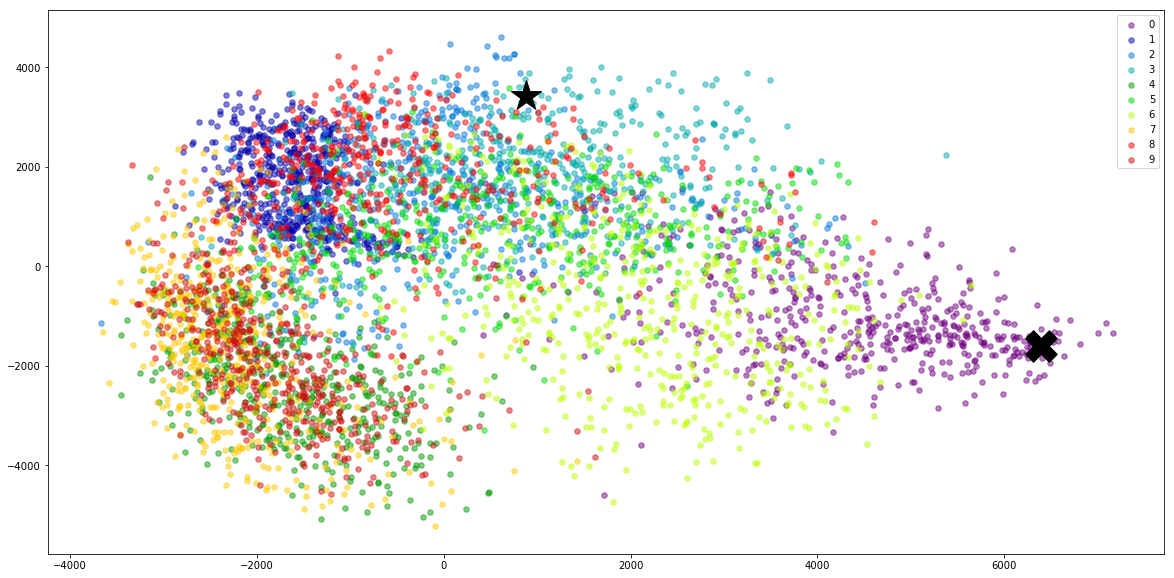
\includegraphics[height=5cm,width=5cm]{./Figures/SE_OS.png}
\caption{SE}
\end{subfigure}\hspace*{\fill}
\begin{subfigure}{0.32\textwidth}
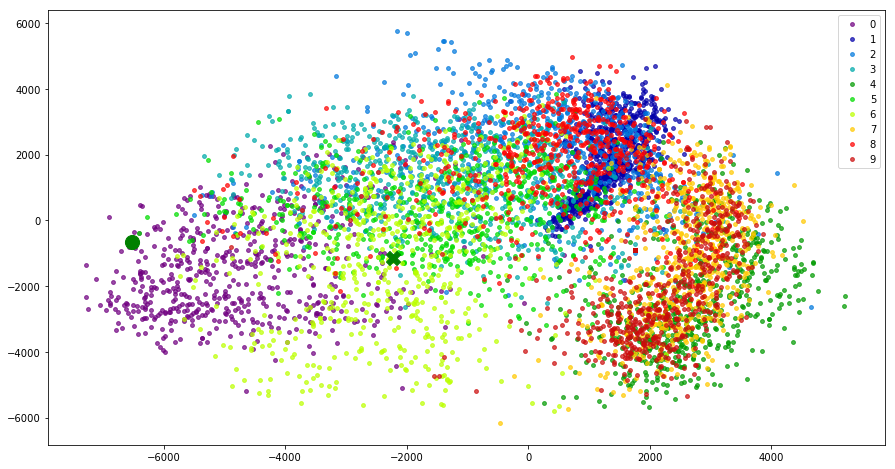
\includegraphics[height=5cm,width=5cm]{./Figures/TSNE_OS.png}
\caption{TSNE} 
\end{subfigure}

\caption{Out of sample predication for manifold learning algorithms} \label{OSML}
\end{figure}

\subsection{Model and Training}
As the discussed manifold algorithms didn't perform as per our expectation, we using dimension reduction on the original data. The reduced dimension data is the trained via simple to complex supervised algorithms. To perform digit recognition task, we seek help of three basic supervised algorithms:  K-Nearest Neighbour (KNN) \citep{Babu2014} , Support Vector Machine (SVM) \citep{Stein2008} and Convolutional Neural Networks (CNN) \citep{Ah2010}. All the above module is implemented in python where the packages provides great help. 

We also want to compare base model performance with original training data and using reduced dimensions. For example, 200 principle components analysis on our 784 features captures 95\% variability in the data. So by PCA, we build the data sets TRAINpca and TESTpca. Similar procedure is followed for manifold learning algorithms too. By extracting n-components from the low dimension, we build train and text datasets corresponding to manifold learning algorithms. For dimension reduction, we take three manifold algorithms namely Isomap, Locally Linear Embedding and t-distributed Stochastic Neighbor Embedding.

The 5-fold cross validation is performed on the training set comprising of original data and data created out of dimension reduction. Then for every model, we choose the parameters yielding highest cross-validation classification accuracy. We used the chosen parameters to model each algorithm type. Finally, to obtain a real out of sample performance evaluation, we use the best model to predict on the test set. We also want to clarify that, we didn't optimize our model, its basic version only. What we are interested in accuracy of model with dimension reduction in comparison to original dataset.

\subsection{Results}

Our experiments results in implementing three different types of model for four different data sets. For reducing the computational burden, we took subsample of 15,000 from the original training set of 60,000. All the computation was performed on Dell's 7th Generation Intel Core i3-7100H Processor with 16GB DDR4-2400MHz RAM powered with NVIDIA GeForce GTX 960 graphics card. The model with CNN was performed with tensor-flow backed.

As we wanted to compare our models on four different datasets, we first started with original. The training set accuracy with original datasets is summarized in Table \ref{R:ORG}. We hypothesized that a properly trained CNN model to attain highest accuracy, but SVM performed better than CNN. KNN performed as per the expectation.

\begin{table}[ht!]
\caption{Model Summary for $\mathbf{Data}$(original)}
% title of Table
\centering
% used for centering table
\begin{tabular}{c c c }
% centered columns (4 columns)
\hline\hline
%inserts double horizontal lines
Model & Data & Accuracy\\ [0.5ex]
% inserts table
%heading
\hline
% inserts single horizontal line
KNN & original& 91.00 \\
SVM & orignal & 95.60 \\
CNN & orignal & 93.00\\ [1ex]
% [1ex] adds vertical space
\hline
%inserts single line
\end{tabular}
\label{R:ORG}
% is used to refer this table in the text
\end{table}

Taking the results summarized in table \ref{R:ORG}, we trained our three model on the data, where dimension reduction was performed using manifold learning algorithm, Isomap. The result summarized in table \ref{R:ISO} failed to our expectation. There was no improvement in accuracy.


\begin{table}[ht!]
\caption{Model Summary for $\mathbf{Data}$(isomap)}
% title of Table
\centering
% used for centering table
\begin{tabular}{c c c }
% centered columns (4 columns)
\hline\hline
%inserts double horizontal lines
Model & Data & Accuracy (\%)\\ [0.5ex]
% inserts table
%heading
\hline
% inserts single horizontal line
KNN & isomap & 92.00 \\
SVM & isomap & 95.50 \\
CNN & isomap & 93.00\\ [1ex]
% [1ex] adds vertical space
\hline
%inserts single line
\end{tabular}
\label{R:ISO}
% is used to refer this table in the text
\end{table}

The models with subsample data obtained after reducing dimension by TSNE improved accuracy of SVM by little percentage, but nothing concrete can be said seeing result \ref{R:TSNE}.

\begin{table}[ht]
\caption{Model Summary for $\mathbf{Data}$(tsne)}
% title of Table
\centering
% used for centering table
\begin{tabular}{c c c }
% centered columns (4 columns)
\hline\hline
%inserts double horizontal lines
Model & Data & Accuracy\\ [0.5ex]
% inserts table
%heading
\hline
% inserts single horizontal line
KNN & tsne & 92.00 \\
SVM & tsne & 96.00 \\
CNN & tsne & 93.00\\ [1ex]
% [1ex] adds vertical space
\hline
%inserts single line
\end{tabular}
\label{R:TSNE}
% is used to refer this table in the text
\end{table}

The models accuracy was decreased using data from LLE as summarized in table \ref{R:LLE}.

\begin{table}[ht]
\caption{Model Summary for $\mathbf{Data}$(lle)}
% title of Table
\centering
% used for centering table
\begin{tabular}{c c c }
% centered columns (4 columns)
\hline\hline
%inserts double horizontal lines
Model & Data & Accuracy\\ [0.5ex]
% inserts table
%heading
\hline
% inserts single horizontal line
KNN & lle & 90.00 \\
SVM & lle & 91.20 \\
CNN & lle & 91.20\\ [1ex]
% [1ex] adds vertical space
\hline
%inserts single line
\end{tabular}
\label{R:LLE}
% is used to refer this table in the text
\end{table}

\section{Conclusions}
\label{C4:con}
The out of sample predication for manifold algorithms indicates that test points are projected on the corrects clusters of training datasets. But the projection of the test points is not so clear. Separation of some numbers are blurred and not separated accurately on the manifold. The prepossessing using Hough transform didn't improve the accuracy. Contrary to our exception, the CNN model didn't perform better than SVM. There was no substantial improvement in the accuracy of hand written digit recognition with preprocessed data having dimension reduction.

